%----------------------------------------------------------------------------------------
%    PACKAGES AND THEMES
%----------------------------------------------------------------------------------------

\documentclass[aspectratio=169,xcolor=dvipsnames]{beamer}
\usetheme{SimpleDarkBlue}
\usepackage{hyperref}
\usepackage{graphicx} % Allows including images
\usepackage{booktabs} % Allows the use of \toprule, \midrule and \bottomrule in tables
\usepackage{natbib}
\setbeamertemplate{bibliography item}[text]
%----------------------------------------------------------------------------------------
%    TITLE PAGE
%----------------------------------------------------------------------------------------

\title{Empathy in VR}

\author{The Sixth Group}

\date{\today} % Date, can be changed to a custom date

%----------------------------------------------------------------------------------------
%    PRESENTATION SLIDES
%----------------------------------------------------------------------------------------

\begin{document}

\begin{frame}
    \titlepage
\end{frame}

\begin{frame}{Overview}
    \tableofcontents
\end{frame}

% First Teammate
\section{Background}

% Second Teammate
\section{Technology}

% Third Teammate
\section{Applications}
\begin{frame}{Applications}
    \begin{center}
        \Large{Applications of Empathy in VR}\\
        \vspace{0.5cm}
        \normalsize{Jinxian Zhu}
    \end{center}
\end{frame}

\begin{frame}{Applications}
    \begin{columns}[c]    
        \column{0.5\textwidth}
        \begin{center}
            \textbf{\large Professional Training} \\
            \vspace{0.1cm}
            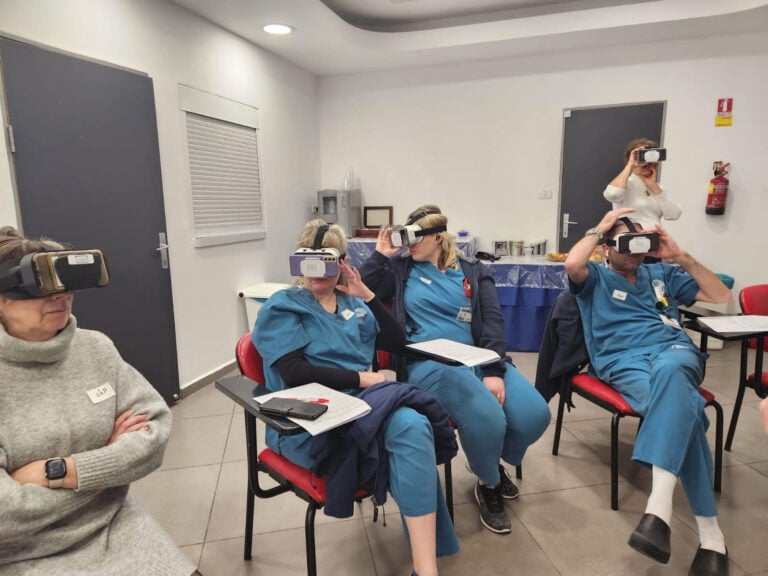
\includegraphics[height=2.8cm]{Pre.-Empathy-in-VR/section3_picture/doctortraining.jpg} \\
            \vspace{0.1cm}
            \begin{minipage}{0.95\textwidth}
                \centering\small
                Enhancing empathy skills of healthcare providers, teachers, and other professionals to improve service quality
            \end{minipage}
        \end{center}
        
        \column{0.5\textwidth}
        \begin{center}
            \textbf{\large Educational Applications} \\
            \vspace{0.1cm}
            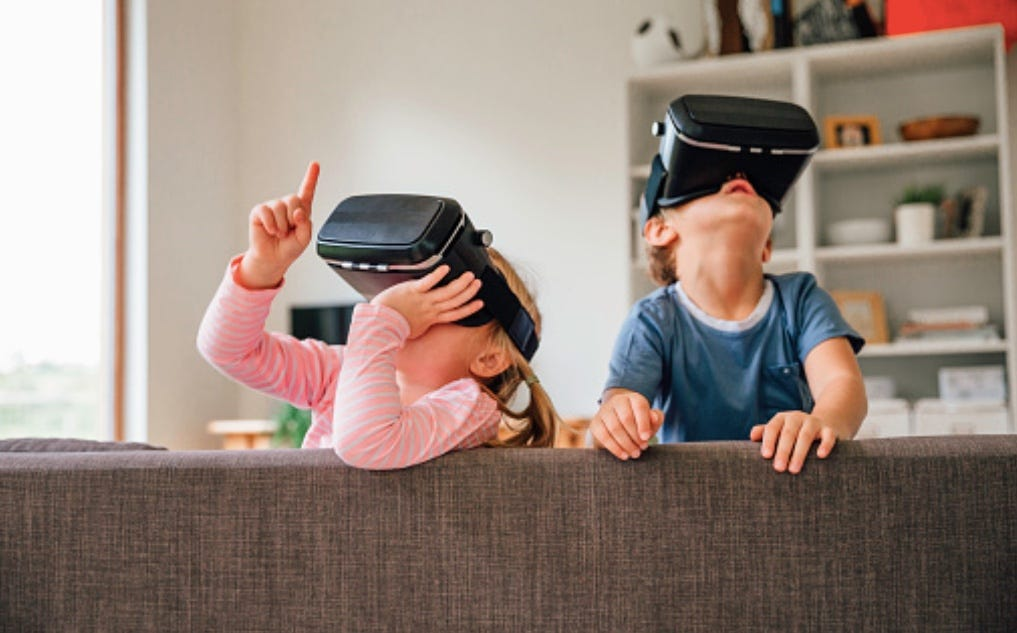
\includegraphics[height=2.8cm]{Pre.-Empathy-in-VR/section3_picture/childrenempathy1.jpg} \\
            \vspace{0.1cm}
            \begin{minipage}{0.95\textwidth}
                \centering\small
                Empathy education for children and the public, promoting social inclusion and diverse understanding
            \end{minipage}
        \end{center}
    \end{columns}
    
    \begin{block}{Application Progress}
        VR empathy applications are transitioning from proof of concept to practical implementation, primarily advancing empathy development through professional training and public education.
\end{block}
\end{frame}

\begin{frame}{VR Empathy in Professional Training: Overview}
    \begin{columns}[T]
        \begin{column}{0.45\textwidth}
            \vbox to 6cm{
                \vfill
                \centering
                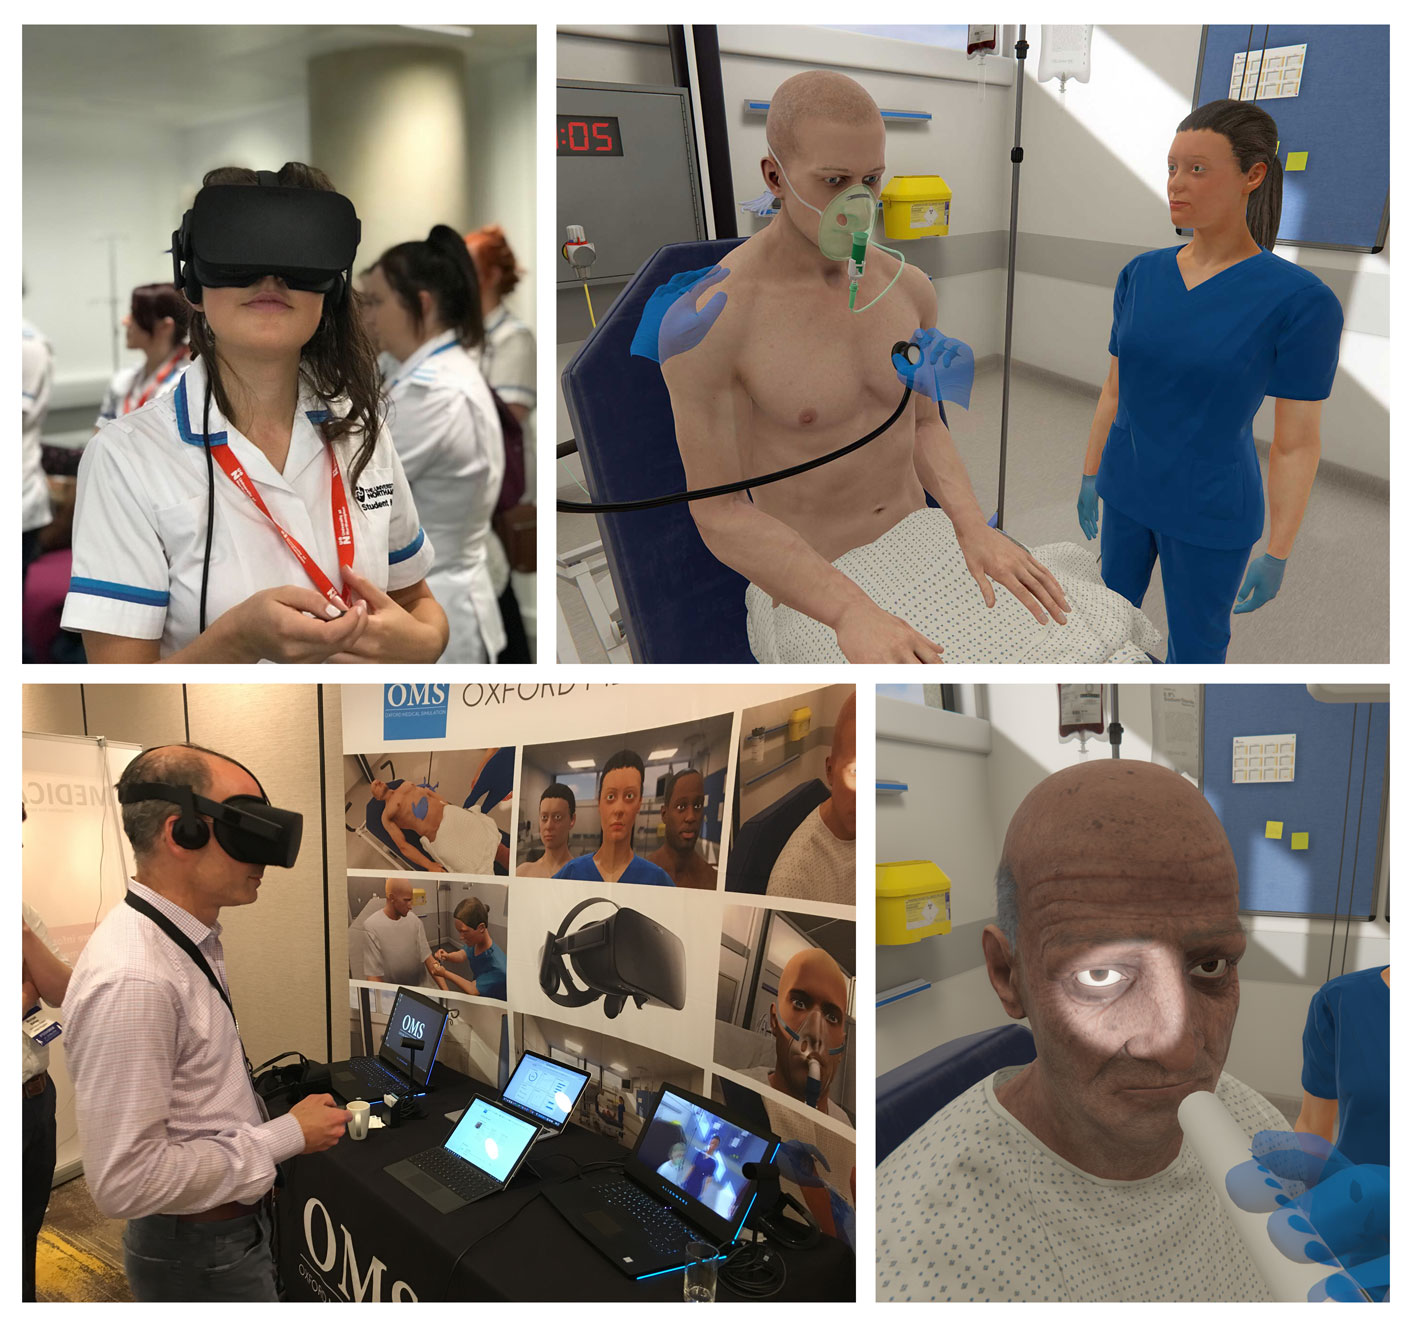
\includegraphics[height=6cm]{Pre.-Empathy-in-VR/section3_picture/medical_training.jpg}
                \vfill
            }
        \end{column}
        
        \begin{column}{0.55\textwidth}
            \vbox to 6cm{
                \vfill
                \begin{block}{Progress of VR Empathy Applications in Professional Training}
                    VR empathy training is transforming professional development by providing immersive perspective-taking experiences that traditional methods cannot replicate.
                    
                    Studies demonstrate VR empathy training produces significant improvements in professional performance metrics and client satisfaction compared to traditional methods.
                \end{block}
                \vfill
            }
        \end{column}
    \end{columns}
\end{frame}



\begin{frame}{Training Objectives \& Theoretical Foundation}
    
    \begin{columns}[c]
        \column{0.5\textwidth}
        \begin{block}{Key Training Objectives}
            \begin{itemize}
                \item Enhance empathic understanding across professional contexts
                \item Develop advanced communication skills for diverse client interactions
                \item Cultivate professional sensitivity to client experiences
                \item Bridge theory-practice gap through immersive learning
            \end{itemize}
        \end{block}
        
        \column{0.5\textwidth}
        \begin{block}{Theoretical Foundation}
            \begin{itemize}
                \item Perspective-taking theory: Understanding others' viewpoints
                \item Embodied cognition: VR facilitates "being in another's shoes"
                \item Emotional contagion: Shared affective experiences
                \item Social presence theory: Immersion enhances empathic response
            \end{itemize}
        \end{block}
    \end{columns}
    
    \begin{alertblock}{Empathy in Professional Settings}
        VR creates unique opportunities for professionals to experience client perspectives firsthand, transforming abstract empathy concepts into embodied understanding that traditional training cannot achieve.
    \end{alertblock}
\end{frame}


\begin{frame}{Applications}
\end{frame}

\begin{frame}{Applications}
\end{frame}

\begin{frame}{Applications}
\end{frame}

\begin{frame}{Applications}
\end{frame}
% Fourth Teammate
\section{Evaluation}

% Fifth Teammate
\section{Challenges}

\end{document}

% %------------------------------------------------
% \section{First Section}
% %------------------------------------------------

% \begin{frame}{Bullet Points}
%     \begin{itemize}
%         \item Lorem ipsum dolor sit amet, consectetur adipiscing elit
%         \item Aliquam blandit faucibus nisi, sit amet dapibus enim tempus eu
%         \item Nulla commodo, erat quis gravida posuere, elit lacus lobortis est, quis porttitor odio mauris at libero
%         \item Nam cursus est eget velit posuere pellentesque
%         \item Vestibulum faucibus velit a augue condimentum quis convallis nulla gravida
%     \end{itemize}
% \end{frame}

% %------------------------------------------------

% \begin{frame}{Blocks of Highlighted Text}
%     In this slide, some important text will be \alert{highlighted} because it's important. Please, don't abuse it.

%     \begin{block}{Block}
%         Sample text
%     \end{block}

%     \begin{alertblock}{Alertblock}
%         Sample text in red box
%     \end{alertblock}

%     \begin{examples}
%         Sample text in green box. The title of the block is ``Examples".
%     \end{examples}
% \end{frame}

% %------------------------------------------------

% \begin{frame}{Multiple Columns}
%     \begin{columns}[c] % The "c" option specifies centered vertical alignment while the "t" option is used for top vertical alignment

%         \column{.45\textwidth} % Left column and width
%         \textbf{Heading}
%         \begin{enumerate}
%             \item Statement
%             \item Explanation
%             \item Example
%         \end{enumerate}

%         \column{.45\textwidth} % Right column and width
%         Lorem ipsum dolor sit amet, consectetur adipiscing elit. Integer lectus nisl, ultricies in feugiat rutrum, porttitor sit amet augue. Aliquam ut tortor mauris. Sed volutpat ante purus, quis accumsan dolor.

%     \end{columns}
% \end{frame}

% %------------------------------------------------
% \section{Second Section}
% %------------------------------------------------

% \begin{frame}{Table}
%     \begin{table}
%         \begin{tabular}{l l l}
%             \toprule
%             \textbf{Treatments} & \textbf{Response 1} & \textbf{Response 2} \\
%             \midrule
%             Treatment 1         & 0.0003262           & 0.562               \\
%             Treatment 2         & 0.0015681           & 0.910               \\
%             Treatment 3         & 0.0009271           & 0.296               \\
%             \bottomrule
%         \end{tabular}
%         \caption{Table caption}
%     \end{table}
% \end{frame}

% %------------------------------------------------

% \begin{frame}{Theorem}
%     \begin{theorem}[Mass--energy equivalence]
%         $E = mc^2$
%     \end{theorem}
% \end{frame}

% %------------------------------------------------

% \begin{frame}{Figure}
%     Uncomment the code on this slide to include your own image from the same directory as the template .TeX file.
%     %\begin{figure}
%     %\includegraphics[width=0.8\linewidth]{test}
%     %\end{figure}
% \end{frame}

% %------------------------------------------------

% \begin{frame}[fragile] % Need to use the fragile option when verbatim is used in the slide
%     \frametitle{Citation}
%     An example of the \verb|\cite| command to cite within the presentation:\\~

%     This statement requires citation \cite{p1}.
% \end{frame}

% %------------------------------------------------

% \begin{frame}{References}
%     \footnotesize
%     \bibliography{reference.bib}
%     \bibliographystyle{apalike}
% \end{frame}

% %------------------------------------------------

% \begin{frame}
%     \Huge{\centerline{\textbf{The End}}}
% \end{frame}

% %----------------------------------------------------------------------------------------